\chapter{Обзор Викиданных}
\label{ch:ReviewAboutWD}

\section{Викиданные}
Викиданные — это структурированная и совместно редактируемая база данных, созданная Фондом Викимедиа\footnotemark \footnotetext{Викиданные (Wikidata) — это свободная, совместно наполняемая, многоязычная, вторичная база данных, в которой собрана структурированная информация для обеспечения поддержки Википедии, Викисклада, а также других вики-проектов движения Викимедиа по всему миру.}. \begin{marginfigure}[0.0cm]
{
	\setlength{\fboxsep}{0pt}%
	\setlength{\fboxrule}{1pt}%
	\fcolorbox{gray}{white}{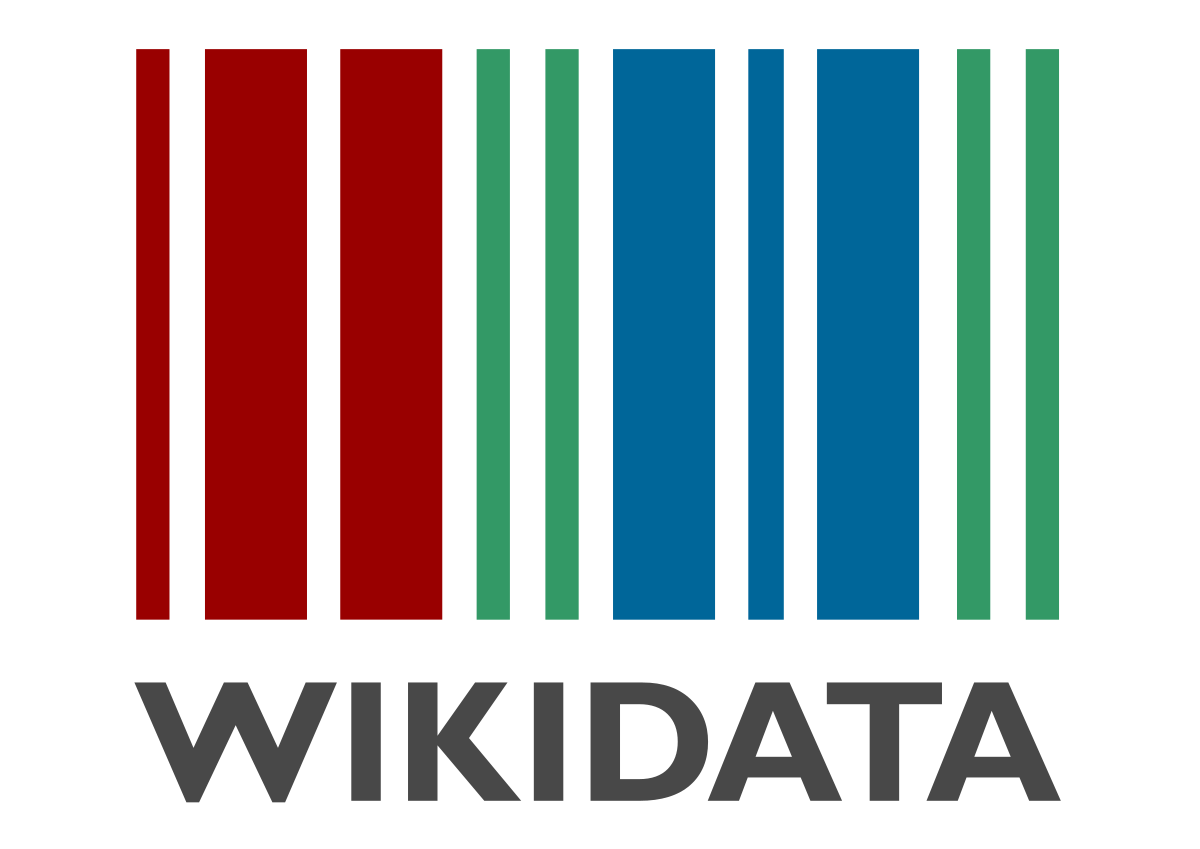
\includegraphics{ru/graphics/chapter/review/Wikidata-logo-en.png}}
}
\caption
{
Логотип Викиданных с текстом на английском языке. \newline
2012 / Planemad
}
\label{fig:seyu}
\end{marginfigure}Проект был официально запущен 30 октября 2012 года, его разработка ведется под руководством Wikimedia Deutschland\cite{Wikipedia_review}. Проект создавался за счёт пожертвований Allen Institute for Artificial Intelligence, Gordon and Betty Moore Foundation и Google. В данный момент Викиданые — это бесплатная и свободная база знаний, которая может использоваться и редактироваться людьми и машинами\cite{Vrandecic}.

Любой объект Викиданных имеет свой уникальный идентификатор и свойства. Эта информация может быть обработана с помощью компьютера, и при этом она понятна пользователям. Сайт Викиданных содержит сервис ‘Wikidata Query’, включающий набор инструментов для построения SPARQL-запросов и их визуализации в виде таблиц, диаграмм, графов или географических карт.

Содержимое Викиданных распространяется по лицензии Creative Commons CC0, которая позволяет повторно использовать информацию самыми разными способами: пользователи могут копировать, изменять, распространять и обрабатывать эти данные в любых целях. Еще одна особенность Викиданных --- это многоязычность. Любой человек может редактировать Викиданные более чем на 350 языках.

Викиданные постоянно обновляются, добавляются новые объекты. На 2021 год насчитывается более 63 миллионов страниц и около 1 миллиарда правок. В 2019 года в Викиданных было совершено более 800 тысяч правок, что превзошло количество правок в английской Википедии и сделало Викиданные наиболее редактируемым сайтом Викимедиа\footnotemark . \footnotetext{Ссылка на веб-сайт Викидынных: \href{https://www.wikidata.org/}{https://www.wikidata.org/}}
\section{Об исследовании Викиданных}
В работе ‘A large-scale collaborative ontological medical database’\cite{Collaborative_ontological_database} описываются плюсы использования Викиданных для создания крупномасштабной совместной медицинской
базы данных. Основные требования к создаваемой базе данных — это платформа с обновлением в реальном времени, подходящая лицензия для последующего использования полученной информации, свободное редактирование на любом языке. Именно это и есть основные характеристики Викиданных. Во-первых, Викиданные — это открытая, редактируемая база знаний. Любой пользователь без навыков программирования может вносить изменения более чем на 350 языках и диалектах. Во-вторых, информация постоянно обновляется, добавляются новые объекты. В настоящее время Викиданные насчитывают более 18000 редакторов. В-третьих, лицензия Creative Commons CC0 обеспечивает широкое использование полученной информации.

Есть несколько альтернативных вариантов баз знаний:
\begin{enumerate}
\item Cyc — проект компании Cycorp (Остин, США) по созданию онтологической базы знаний, позволяющий решать задачи из области искусственного интеллекта\cite{Cyc}. Сейчас Cyc имеет исследовательскую лицензию ResearchCyc. У данной базы знаний есть некоторые недостатки: сложность системы (сложность добавления данных
вручную), недостаток документации для изучения системы, неполнота системы.
\item Evi (ранее True Knowledge\cite{True_Knowledge}) – технологическая компания в Кембридже (Англия), которая специализируется на базе знаний и программном обеспечении семантического поиска. Добавление информации в базу знаний осуществляется двумя способами: импорт из «заслуживающих доверия» внешних баз данных (например: Википедия) и из представления пользователей в соответствии с единообразным форматом и подробным процессом ввода. Как и в Википедии, пользователь может изменять
данные, «соглашаться» или «не соглашаться» с информацией, представленной True Knowledge. Система может отклонить любые факты, которые семантически несовместимы с другими утвержденными знаниями, в отличие от Викиданных, где могут
храниться противоречивые данные.
\end{enumerate}
По мнению авторов статьи, Викиданные являются лучшим вариантом для обработки информации, т.к. можно связывать объекты через их свойства (экземпляр P31, подкласс 279, часть P361, имеет часть P527), создавать SPARQL-запросы, визуализировать их результаты в виде таблиц, графов, диаграмм или сохранять в нужном формате (CSV, JSON, SVG).

Таким образом, авторы призывают обратить внимание на Викиданные, которые могут взять на себя роль централизованного хранилища данных. В статье ‘Falcon 2.0: An Entity
and Relation Linking Tool over Wikidata’ \cite{Falcon_2.0} приводится пример использования Викиданных в качестве централизованной и общедоступной базы знаний для системы FALCON 2.0. Это инструмент, связывающий сущность и отношения через Викиданные. Эта система идентифицирует сущности в коротком тексте или вопросе, а затем связывает их с соответствующими URL в графе знаний Викиданных.